%!TEX root = paper.tex
\section{BLE PHY-layer Fingerprinting}
\label{sec:methodology}

In this section, we present a new physical layer fingerprinting technique that
can uniquely identify BLE devices.
%
We first describe why surprisingly, even though BLE signals are much less
complex than WiFi, many mobile devices introduce the  same complex hardware
imperfections in BLE as they do in WiFi.
%
Then we present a new algorithm to robustly and accurately extract these
WiFi-like imperfections from BLE packets.
%
The key contribution of our algorithm is overcoming the primary limitation of
BLE physical layer fingerprinting: its short known samples in its preamble
(Section~\ref{sec:motivation:diff}).

\subsection{BLE has WiFi-like signal imperfections} %{{{

\begin{figure}[t!]
    \centering
    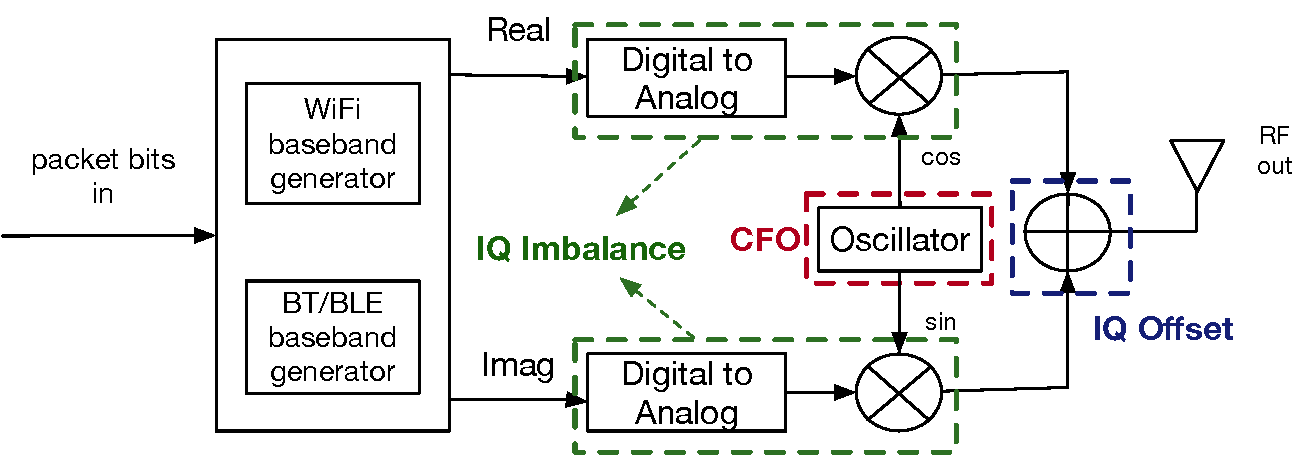
\includegraphics[width = \linewidth]{plots/IQchain.pdf} 
    \caption{Architecture of WiFi/BLE combo chipsets}
    \label{fig:iq_arch}
\end{figure}


WiFi chipsets have a unique fingerprint because they require generation of
complex multi-carrier modulation waveform. To generate this waveform, many
mobile device chipsets use an I/Q modulation architecture shown in
Figure~\ref{fig:iq_arch}.
%
The hardware imperfections in the I/Q architecture include the following:
\emph{Carrier Frequency Offset (CFO)} and \emph{IQ imperfections} (which
consists of IQ offset and IQ imbalance). \emph{CFO} is the error in the carrier
frequency fed to the mixer. It is caused by imperfections in the radio's
crystal oscillator; specifically, the crystal and the tolerance of oscillators
yields unique CFO even the devices from the same make and model.
%
The \emph{IQ imperfections} result from the following phenomenon: IQ offset is
comes from the center carrier leaking into the signal, or the baseband signal having a
DC offset.% This can add a fixed complex term to the I and Q sample (shift the
%center of constellation).
IQ imbalance occurs because of a mismatch
between parallel analog components of RF chain in I (in-phase) and Q
(quadrature) signal path.% This makes the phase and amplitude of I and Q path
%asymmetric. 

%In this type of
%transmitter, the I (real) and Q (imaginary) parts of the waveform are generated
%by the digital baseband. The real and imaginary parts of the signal are
%eventually mixed with a carrier frequency ($f_c$), where real part is
%multiplied cosine ($cos(2\pi f_c t$) of the carrier frequency and vice versa
%for imaginary part.

\subsubsection*{Mobile devices use combo BLE/WiFi chips}
%
In order to save cost of RF hardware, high power devices (e.g. smartphones) are
equipped with combo chips which have both BLE and WiFi digital baseband, and
share the same I/Q front-end 
(Figure~\ref{fig:iq_arch}).
%
Combining these protocols reduces the device's overall size, and serves as a
point to synchronize both protocols' 2.4~GHz transmissions so they do not
interfere with each other.
%
However, an unintended result of this hardware design choice, is that BLE
transmissions contain the same imperfections that can fingerprint
WiFi transmitters.


%}}}

\subsection{Estimating CFO\&I/Q imperfections in BLE} %{{{
\label{sec:methodology1}
%
%These hardware imperfections have been demonstrated to be the most important
%characteristics for building RF fingerprinting systems for WiFi devices.  As a
%result, we can take advantage of these previously explored hardware
%imperfections to build our physical layer attack on BLE devices.
%
Although combo chips introduce WiFi-like imperfections in BLE transmissions
from mobile devices, estimating these imperfections in a capture of a BLE
transmission is extremely challenging (Section~\ref{sec:motivation:diff}).
%
%There is no existing technique for estimating the mentioned imperfections for
%BLE devices with the granularity and accuracy which is needed for the task of
%device identification.
%
%
First, we describe how typical BLE receivers perform limited, course grained,
estimation and removal of physical-layer imperfections.
%
Then we present a new BLE fingerprinting algorithm that can estimate these
imperfections accurately and robustly.

%As discussed in Section~\ref{sec:background}, CFO, IQ offset and IQ imbalance
%are important hardware characteristics that can be leveraged to uniquely
%identify this architecture as proposed by prior works for fingerprinting WiFi
%devices as well. However, the challenge is how we can estimate these
%imperfection parameters accurately and fine-grained to fulfill the device
%identification task. WiFi signal eases this job by having specific signal
%features such as LTF and multiple subcarriers (and also WiFi chipsets report
%CSI which can easily be used to estimate these imperfections). This is mainly
%because fine-grained estimation and compensation of CFO and IQ imperfections is
%an unavoidable step in decoding WiFi signal. If CFO compensation is not
%accurate in WiFi decoding, IQ samples will rotate by time, and if IQ
%imperfection is not compensated, the shape of constellation will change. Both
%of these will drastically affect the decoding process since symbols are
%modulated in IQ domain. As a result, the mentioned signal features have been
%anticipated and there is a huge body of work on how to etimate these
%imperfections accurately for WiFi signals (not only for RF fingeprinting, but
%also for other purposes).


%In order to build a robust algorithm, we would start from the physics of the
%BLE architectures and build algorithms to capture hardware impariments to
%uniquely identify each radio. We present a novel algorithm to recover the
%hardware impairments which WiFi based RF fingerprinting relies on.
%Specifically, we would discuss how to extract the accurate hardware
%impairments such as CFO, IQ offset and IQ imbalance with just using the BLE
%transmissions which have narrow bandwidth with short packet sizes and short
%preamble length. 

%Next, we un-cover that not all devices use IQ architecture or popular architecture used by WiFi transceivers. In order to reduce power, the  reveal that BLE-only chipsets do not use the commonly known transmitter architecture and consequently, do not have many of the well-known hardware impairments. As a result, we porpose a new technique for profiling those architectures. Finally, we illustrate the overall flow of our fingerpriting methodology.
\begin{comment}
and we show that the second technique can be used to fingerprint any kind of bluetooth transmitter, regardless of the transmitter architecture.
\end{comment}

%Hardware Impairment estimation for WiFi/BLE Combo-chips}

% Talk about the combo chip first and explain how smartphone use those and therefore we can use the similar hardware impariments as IQ chipsets.

% this sentence says everything in one sentence slow it down, talk about WiFi devices first, show a figure with the architecture of the WiFi chipset to explain

%Practical hardware concerns have made the usage of I/Q path in transmitter architecture including WiFi chipsets, a desirable choice. In this kind of architecture, I and Q data are generated in different paths and eventually they are mixed with the carrier frequency. On the other hand, the hardware imperfections caused by this kind of hardware design, including CFO, IQ offset and IQ imbalance [CITE], have been proposed as important hardware characteristics which can be used to distinguish different devices. Naturally, the devices equiped with both BLE and WiFi technology (e.g. smartphones), utilize the same piece of hardware as a combo chipset for sending both BLE and WiFi packets as shown in Fig. XXXX. The reason lies in cost efficiency, simplifying board design, and optimizing die size and on-board area. As a result, we can take advantage of previously explored hardware imperfections (CFO, IQ offset and IQ imbalance). \\

%In previous works, CFO, IQ offset and IQ imbalance [CITE] have been proposed as important hardware characteristics which can be used to distinguish different devices. 


% Next talk about WiFi decodes the CFO etx and how it does, can we apply similar technique to BLE, we cannot, why?
% talk about how BLE is challenging with narrow bandwidth, short preamble makes it hard to detect CFO, if similar techqnieu as WiFi is applied what is the resolution you would get and would it resolve the devices (make the problem look hard)

%Measuring these harware imperfections is an unavoidable stage in decoding WiFi packets since it can significantly affect the decoding error if the receiver does not compensate them. As a result, measuring these imperfection has been heavily researched for WiFi signals. More than that, pecific arrangements have been devised in WiFi protocol to make the estimation of these imperfections easy and accurate. On the other hand, decoding the simple GFSK modulation which is used in BLE and Bluetooth, is not affected by the aforementioned imperfections severly. Therefore, there has not been any attempt on measuring these impairments accurately for a BLE or Bluetooth signal. Also, using the same techniques for estimating impairments as WiFi, will result in a much lower accuracy of estimation because of having a narrowband (without subcarrier) short signal (typically a few hundreds of microseconds) with a very short premble (8 microseconds). For instance, we employed the technique that is used in Bluetooth test equipments which exploits the preamble to estimate CFO [CITE]. That is, simply we take the average of frequencies in the preamble. Since preamble is an 8-bit sequence of consecutive 0 and 1, the frequency of preamble is symmetric. Therefore, ideally the average of thh frequencies in preamble must be 0. If there exists CFO, this average will be an estimate of CFO. However, this estimation is not precise and robust as it only relies on a an 8-microsecond preamble. The resulting standard deviation of the measured CFO was 1.5 KHz (we averaged the CFO standard deviation across 20 different devices). This standard deviation is huge for performing the task of RF fingeprinting and will end up in low accuracy of identifying devices based on RF fingerprints. We also tried the MINMAX algorithm described in [CITE] but it yields even worse standard deviation.\\

% then propose your solution layer by layer, first layer to increase the resolution your idea is to use entire packet, which requires you to decode the data and then reconstruct the receive singal witout hardware impariment and use that to estimate the impariements. 

%In WiFi it is necessary 
%features such as LTF and multiple subcarriers (and also WiFi chipsets report
%CSI which can easily be used to estimate these imperfections). This is mainly
%because fine-grained estimation and compensation of CFO and IQ imperfections is
%an unavoidable step in decoding WiFi signal. If CFO compensation is not
%accurate in WiFi decoding, IQ samples will rotate by time, and if IQ
%imperfection is not compensated, the shape of constellation will change. Both
%of these will drastically affect the decoding process since symbols are
%modulated in IQ domain.

% Extra text {{{
\if 0
Unlike WiFi, decoding BLE or Bluetooth signals does not require accurately
estimating and compensating for CFO and IQ imperfections.
%
Even several KHz of CFO will not affect the decoding process of BLE's FSK
signals. Also, as FSK symbols are not modulated in IQ domain, IQ imperfections
does not significantly the affect BLE decoding process.
%
As a result, unlike WiFi, there was no need to embed any known signal feature
in BLE signal to provide necessary means for accurate and fine-grained
estimation of these imperfections.
%
For instance, BLE preamble is only 8 bits (8 microseconds) which is much
shorter than WiFi, it uses the simple GFSK modulation, and there does not
exists multiple subcarrier in BLE signal or CSI in BLE chipsets. These
simplicities of BLE signal leaves us in a situation where estimating these
imperfections for BLE signals is much more challenging than WiFi.
The consequence of this fact is that existing techniques for fine-grained
estimation of CFO and IQ imperfection of WiFi signals, either cannot be
adopted or will not result in fine-grained imperfection estimation for BLE
signals.  Moreover, techniques that are specifically designed for CFO
estimation of BLE or Bluetooth signals provides only a very coarse-grained
estimation which is not sufficient for device identification task at all, and
not surprisingly, there has not been any attempt on estimating IQ imperfection
for BLE or BLuetooth signals as it is not needed for decoding.
\fi
%}}}

\vspace{0.5em}
\noindent\textbf{Existing coarse CFO estimation in BLE receivers}
Coarse-grained CFO compensation is implemented in BLE receivers.  They
implement this by analyzing the small number (8) of known samples in the
preamble of each packet.
%
BLE receivers estimate CFO from these bits by averaging the frequencies of each
FSK symbol in the preamble. Another popular CFO algorithm used in the Texas
Instruments CC2400 BLE chipset averages the minimum and maximum frequency of
the preamble~\cite{cvtracksun}.
%
Since the preamble is an 8-bit sequence of consecutive 0 and 1, the frequency
of preamble is symmetric.  Therefore, ideally the average of the frequencies in
preamble must be 0. If there exists CFO, this average will be an estimate of
CFO.
%
However, as these techniques only rely on 8 samples, they do not produce an
accurate estimate of CFO---leading to confusions between device fingerprints.
%
Indeed, with only 8 samples, the theoretical limit of CFO accuracy 2 KHz assuming 3 degree
phase noise.
%

%
% ADS: Sounds fun but no space
%
%We tried simply extending this method to take advantage of the entire packet
%and take average across frequencies of equal number of 0's and 1's. However,
%we did not see any significant benefit for doing that.

\subsubsection{Goals}
%
To implement an improved BLE CFO fingerprinting algorithm, and to estimate I/Q
in addition our algorithm must have two key properties.
%
First, instead of relying on the 8 known samples in the preamble, our goal is
to utilize the entire packet ($\sim$370 samples).
% in order to diminish the
%effect of noise and provide more information and granularity for accurate
%imperfection estimation.
These additional samples will provide a theoretical CFO accuracy of 
11 Hz compared to the 2 KHz of coarse-grained
estimation.
%
Second, it must jointly estimate CFO and I/Q imperfections to prevent the
mutual effects on each other's estimation.

\subsubsection{Overview}
%
Keeping these two goals in mind, we develop an algorithm to estimate CFO and IQ
imperfections for BLE signals.
%
To be able to take advantage of the entire packet properly, we need to first
decode the packet. Our insight is that because GFSK modulation is very robust,
we will be likely to decode the packet correctly, and this can be checked with
BLE's CRC.
%
Once we have the decoded data, we can reconstruct an ideal perfect version of
the transmitted signal.
%
Then we jointly insert the hardware imperfection parameters (CFO and I/Q) in the
mathematical model of the ideal signal. Then we keep modifying those
imperfection parameters until the ideal representation of the signal
looks like the actual captured signal. However, since the search space for
these imperfection parameters is vast, we use optimization techniques to
efficiently move towards the optimal value of parameters.

%to WiFi. Therefore, decoding can be done properly without compensating hardware
%imperfections.  

%However, to build an algorithm for estimating these fingerprints accurately and robustly, despite the existing techniques, we cannot rely on the preamble since it is very short for BLE and also, there is no notion of subcarrier in BLE technology. For instance, we employed the technique that is used in Bluetooth test equipments which exploits the preamble to estimate CFO~\cite{?}. That is, simply we take the average of frequencies in the preamble. Since preamble is an 8-bit sequence of consecutive 0 and 1, the frequency of preamble is symmetric. Therefore, ideally the average of the frequencies in preamble must be 0. If there exists CFO, this average will be an estimate of CFO. However, this estimation is not precise and robust enough as it only relies on a an 8-microsecond preamble. The resulting standard deviation of the measured CFO was 1.5 KHz (we averaged the CFO standard deviation across 20 different devices). This standard deviation is huge for performing the task of RF fingeprinting and will end up in low accuracy of identifying devices based on RF fingerprints. \\

%Instead of relying on preamble or specific short parts of the packet, we can benefit from the entire packet to make a robust and accurate imperfection estimator since using the entire packet helps in diminishing the effect of noise as well as providing more information and granularity to estimate imperfections accurately. Although for being able to take advantage of the entire packet properly, we need to first decode the packet. Note that thanks to simple GFSK modulation, hardware imperfection does not cause decoding error as opposed to WiFi. Therefore, decoding can be done properly without compensating hardware imperfections. Once we have the decoded data, we can reconstruct the ideal signal. The high level idea is that we insert hardware imperfection parameters in the mathematical model of the ideal signal. Then we keep changing those imperfection parameters until the mathematical representation of the signal looks like the actual captured signal. However, since the search space for these imperfection parameters is vast, we use optimization techniques to move towards the optimal value of parameters efficiently. \\
%Although we consider GFSK modulation in this paper, the idea behind this method can be extended to many other modulation schemes. 

% estimating impariments is not easy, explain the math model and explain why it is hard, as it not convex 

% present your insights to use a gradient descent algorithm, however even that gets stuck at local minima's which is not great, so you fix this by choosing right intial value. 

% explain how you choose right initial value, what are your insgihts and why does those work. 

% finally show the performance of your algorithm before ending the section. 




\begin{comment}
    To measure these hardware impairments, we mathematically model them and then use optimization techniques to estimate these imperfections. 
\end{comment}

\subsubsection{Jointly estimating CFO and I/Q}

Let $y = Real\{y\}+jImag\{y\}$ be the captured baseband signal (normalized by the average amplitude). In a GFSK modulated signal, ideally we have $Real\{y\} = cos(\omega(t)t)$ and $Imag\{x\} = sin(\omega(t)t)$ where $\omega(t)$ is the baseband frequency of the signal which is generated according to the GFSK modulation. However, the aforementioned hardware imperfections will slightly change the signal. We first decode the signal to obtain the sequence of bits and then, we make $\omega(t)$ according to GFSK modulation. Let $y'$ be the model of the imperfect signal. Considering the effects of CFO, IQ offset and IQ imbalance, we can write
\begin{gather*}
    y'(t) = \big[(A-\frac{\epsilon}{2})cos(\omega(t)t-\frac{\phi}{2})+I+ \\
    j\big((A+\frac{\epsilon}{2})sin(\omega(t)t+\frac{\phi}{2})+Q)\big)\big]e^{j(\phi_o+2\pi f_o t)}
\end{gather*}
where $f_o$, $\phi_o$, $A$, $\frac{\epsilon}{A}$, $\phi$, $\frac{I}{A}$ and $\frac{Q}{A}$ denote CFO, phase offset, normalized amplitude of the signal, IQ amplitude imbalance, IQ phase imbalance, I offset and Q offset, respectively. The goal is to choose the value of these variables in such a way that $||y'-y||^2$ is minimum and as a result, $y'$ is as close as possible to the captured signal $y$. Therefore, we must solve the following optimization problem:
\begin{gather*}
    min_{f_o,\phi_o,A,\epsilon,\phi,I,Q}{F=||y'-y||^2 =} \\ |Real\{y'\}-Real\{y\}|^2+|Imag\{y'\}-Imag\{y\}|^2
\end{gather*}
However, this problem is not convex. Consequently, any optimization technique may end up in a local optima. To avoid this, we initialize the variables properly to increase the chance of finding the global minimum significantly. Although theoretically it will not guarantee ending up in the global minimum for arbitrary optimum numbers of these variables, we found that in practice we will reach the optimum value with this initialization in practical conditions. 

To initialize CFO, start by taking the average of frequencies in the preamble. Then we compensate the initial CFO in the signal to get the signal $z = y e^{-2\pi f_o t}$. To estimate initial I/Q imperfections, we use the I/Q constellation of the GFSK signal. The I/Q constellation of an ideal GFSK signal is a circle centered at $(0,0)$ since the phase changes according to GFSK modulation but the amplitude is always constant. However, I/Q imperfection will change this constellation. Specifically, I/Q offset will shift the center of the circle as it is equivalent to adding a fixed complex term to the ideal signal, and IQ imbalance will change the shape from a circle to a tilted ellipse.
%
%These effects are shown in Figure~\ref{fig:iq_const}.
As a result, to get an initial estimation of IQ imperfections, we fit an ellipse to the 2-dimensional points $(Imag\{z\},Real\{z\})$ by minimizing the Least Square Error. The center of the ellipse will provide the initial IQ offset and initial IQ imbalance can be obtained from the ratio of minor and major diameter and rotation angle of the ellipse.\\

\if 0
\begin{figure}[t!]
    \centering
    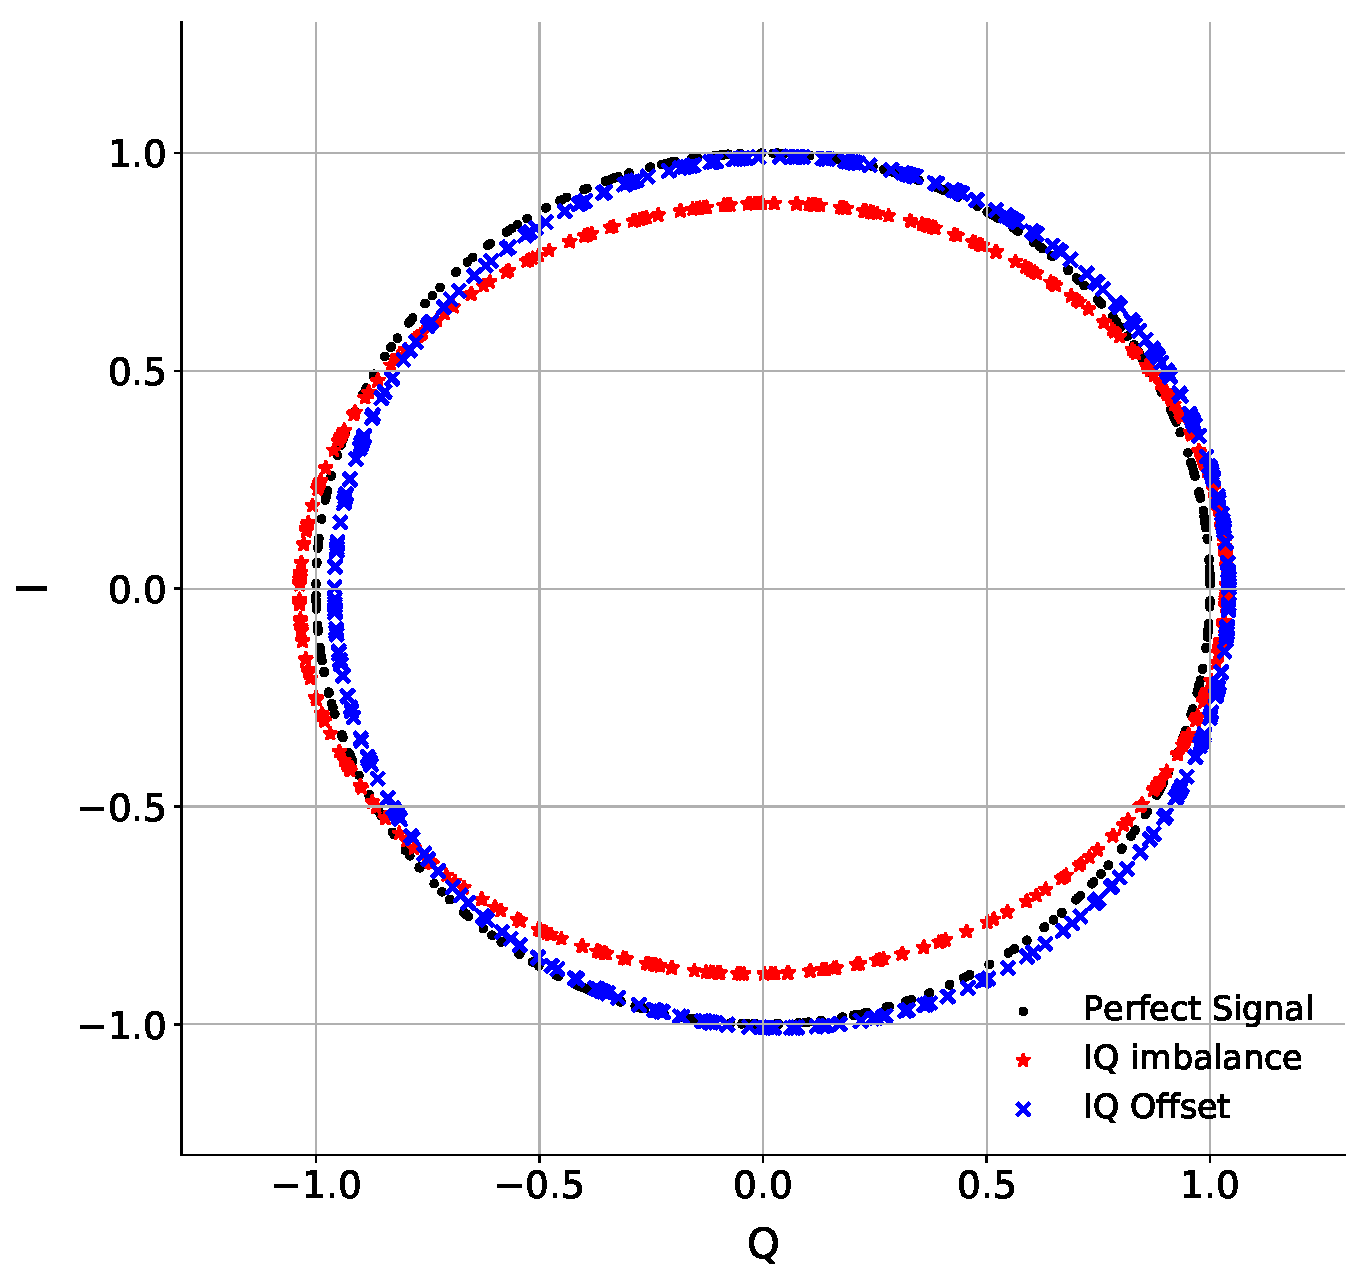
\includegraphics[width = \linewidth]{plots/IQ_const.pdf} 
    \caption{Effects of IQ imperfection on IQ constellationo of a GFSK signal without noise and CFO}
    \label{fig:iq_const}
\end{figure}
%it will be long if I want to explain this ellipse thing
\fi

Although, these initial estimations provide an initialization close to optimum,
they are not accurate. As mentioned earlier, this initialization of CFO
is not accurate and robust enough as it only relies on an 8-microsecond
preamble. Also, mismatch in CFO compensation will cause a time-dependent phase
shift which distorts the I/Q constellation. Therefore, the initial IQ offset
and imbalance estimation will also have errors. Consequently, we employ
optimization techniques to jointly estimate hardware imperfection parameters
precisely and robustly. Therefore, after this initialization, we use Nesterov
Accelerated Gradient Descent (NAG) to move towards the optimum values
of $f_o,\phi_o,A,\epsilon,\phi,I,Q$ by minimizing $F$ in the mentioned
optimization problem.

% TOO LONG ====================
%However, as mentioned earlier, this optimization problem is convex and we may converge to the local optima. Therefore, if after convergence, the average of $F$ was not less than a certain threshold which is determined according to SNR, we add certain steps to the first initialization and repeat the aforementioned gradients descent process. We keep searching for the optimum with new initializations until either the average of $F$ falls below the threshold or our initialization falls out of the bound of the typical values for these imperfections (in which case we give up on the packet. This typically happens when the SNR is less than 5 dB or there is a collision). The first initialization will increase the speed of convergence as usually it will be close to the optimum and re-initialization will ensure ending up in a point which is either the global optimum or very close to global optimum (in the sense that the objective function is less than the desired threshold and hence, is within a small margin of global optimum). The proposed algorithm fulfills the two key properties that we explained at the beginning of this subsection. First, the NAG based joint estimation of CFO and IQ imperfections ensures precise estimation with fine granularity as it keeps moving towards the optimum with adaptive steps and removes the mutual effect of mismatch in estimating these imperfection parameters. Second, the objective function of optimization is chosen as the summation of all PHY samples across the packet, which diminishes the impact of AWGN and provide more robust information and granularity. The final result is achievement of a highly precise CFO and IQ estimates for a device, that are robust to environmental noise, and can therefore be used by an attacker as a unique fingerprint for generic consumer devices.
% Shorter ==========
However, as mentioned earlier, this optimization problem is not convex and we may converge to the local optima. Therefore, if after convergence, the average of F was not less than a certain threshold which is determined according to SNR, we add certain steps to the first initialization and repeat the aforementioned gradients descent process. The proposed optimization based estimation ensures precise estimation with fine granularity as it keeps moving towards the optimum with adaptive steps and removes the mutual effect of mismatch in estimating these imperfection parameters. Moreover, the objective function of optimization is chosen as the summation of all PHY samples across the packet, which diminishes the impact of AWGN and provide more robust information and granularity.

% This is restated, so cutting other eval is there now
\if 0
We use this methods to extract CFO, IQ offset and IQ imbalance for 20 ESP32 chipsets of the same make and model. Figure~\ref{fig:esp} represents CFO and IQ offset magnitude for 10 packets for each of these 20 chipsets. The low variance of CFO for each device, shows this methods is very precise in measuring hardware imperfections (e.g. the CFO standard deviation average for 20 devices is 200 Hz in our algorithm which is significanly less than the existing methods described earlier). Obviously, low within-class variance will significantly improve the identification accuracy and these 20 devices can be clearly distinguished only by their CFO and IQ offset. 
\fi

\vspace{0.5em}
\noindent\textbf{Summary:} For the first time we showed that it is feasible to estimate CFO and IQ imperfections of WiFi/BLE combo chipsets based on the simple BLE signal itself; in other words, without needing the rich signal features that are present in WiFi.


\subsubsection{Profiling and identifying the device}
\label{sec:methodology2}

The first step in deploying our RF fingerprinting attack is to capture the BLE signal. We use an SDR to capture raw I and Q samples of BLE. Next, we use the captured signal to fingerprint the device. The entire processing flow can be divided into two stages, Fingerprinting Stage and Identification Stage. In the former stage, the device is isolated and we capture a number of packets from the target device to build a profile for the device (training packets). The latter stage, employs this profile to identify the device when the MAC addresses is changed.

\vspace{0.5em}
\noindent\textbf{Fingerprinting Stage:} For each packet from a device $D$, CFO and IQ imperfections can be extracted with a high resolution using algorithm described in~\ref{sec:methodology1}. Let $x_1,...,x_N$ be the CFO and IQ imperfection feature vectors for $N$ training packets we have received from device $D$. We calculate the mean $\mu_D$ and covariance matrix $\Sigma_D$ of $X = [x_1 \quad ... \quad x_N]$. $\mu_D$ and $\Sigma_D$ together with a threshold that will be defined later is considered the profile of device $D$.

\noindent\textbf{Identification Stage:} In identification stage, we want to decide whether a packet $x_t$ with a new MAC address belongs to device $D$, indicating that the target device is present. To do so, we compute the Mahalanobis distance to the profile of device $D$

\begin{gather*}
    distance(x_t,\mu_D,\Sigma_D) = \sqrt{(x_t-\mu_D)^T\Sigma_D^{-1}(x_t-\mu_D)}
\end{gather*}


This distance is a way to measure how close the features of the new packet are to the profile of device $D$. In addition to $\mu_D$ and $\Sigma_D$, we define a threshold $thresh$ as the profile of the device. Whenever $distance(x_t,\mu_D,\Sigma_D)<thresh$, packet $x_t$ belongs to the target device $D$ and device $D$ is identified. Otherwise, packet $x_t$ belongs to some other device in the world that we are not looking for. This threshold is chosen using the validation set.
Moreover, since the MAC address is fixed for a period of time, we receive a number of packets with the same MAC address which we know belong to the same device. As a result, we can make a decision about the identity of the MAC address instead of the individual packets. One way that we found most effective, was to first average the feature vector $x$ for all packets with the same MAC address and then compute the Mahalanobis distance. This would further reduce the tolerance due to estimation error and inherent tolerance of features.

\if 0 % extra {{{
\paragraph{Fingerprinting Stage} For each packet from a device $D$, CFO anf IQ imperfections (IQ offset and IQ imbalance) can be extracted with a high resolution using algorithm described in~\ref{sec:methodology1}. Let $x_1,...,x_N$ be the CFO and IQ imperfection feature vectors for $N$ training packets we have received from device $D$. We calculate the mean $\mu_D$ and covariance matrix $\Sigma_D$ of $X = [x_1 \quad ... \quad x_N]$. $\mu_D$ and $\Sigma_D$ together with a threshold that will be defined later is considered as the profile of device $D$.



%Note that IQ offset and imbalance are only useful for combo transmitters and will be ignored by classifier while classifying BLE-only transmitters.
\paragraph{Identification Stage} In identification stage, we want to decide whether a packet $x_t$ with a new MAC address belongs to device $D$, indicating that the target device is present. To do so, we compute the Mahalanobis distance to the profile of device $D$

\begin{gather*}
    distance(x_t,\mu_D,\Sigma_D) = \sqrt{(x_t-\mu_D)^T\Sigma_D^{-1}(x_t-\mu_D)}
\end{gather*}
\begin{gather*}
    distance(x_t,\mu_D,\Sigma_D) = \sqrt{(x_t-\mu_D)^T\Sigma_D^{-1}(x_t-\mu_D)}
\end{gather*}
%This is assuming that the estimated CFO and IQ imperfections have a Gaussian distribution which is a fair assumption considering that the tolerance in CFO and IQ imperfection estimation of a device for different packets is mainly caused by variations in SNR (which affects estimation error) and tolerance of the underlying hardwar.
This distance is one way to measure how close the features of the new packet are to the profile of device $D$. In addition to $\mu_D$ and $\Sigma_D$, we define a threshold $thresh$ as the profile of the device. Whenever $distance(x_t,\mu_D,\Sigma_D)<thresh$, packet $x_t$ belongs to the target device $D$ and device $D$ is identified. Otherwise, packet $x_t$ belongs to some other device in the world that we are not looking for. This threshold is chosen using the validation set.
Moreover, since the MAC address is fixed for a period of time, we receive a number of packets with the same MAC address which we know belong to the same device. As a result, we can make a decision about the identity of the MAC address instead of the individual packets. One way that we found most effective, was to first average the feature vector $x$ for all packets with the same MAC address and then compute the Mahalanobis distance. This would further reduce the tolerance due to estimation error and inherent tolerance of features.


\fi
%}}}

\subsubsection{Comparing CFO accuracy} %{{{
\begin{figure}[t!]
    \centering
    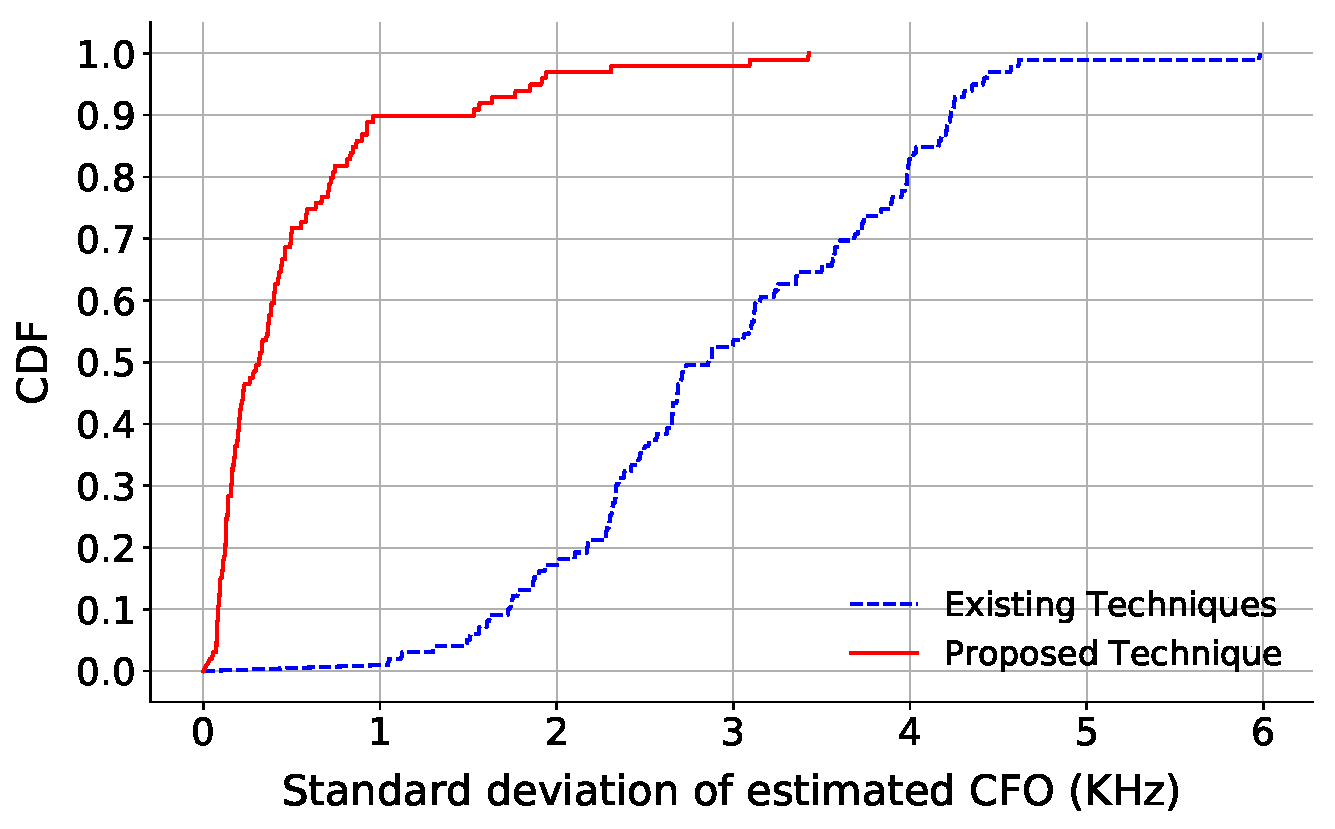
\includegraphics[width = \linewidth]{plots/CFO_comparison_ESP.pdf} 
    \caption{Comparing the CFO estimation of existing coarse-grained techniques with our proposed technique.}
    \label{fig:cfo_comp}
\end{figure}


%
To evaluate the accuracy of our new fine-grained fingerprinting algorithm compared to coarse-grained BLE
CFO estimation, 
we compute CFO for 100 packets from 100 of BLE transmitters observed in the field.% For each device, we
%consider the CFO estimation technique which yielded the lowest standard deviation (std).
%
Figure~\ref{fig:cfo_comp} shows the CDF of the standard deviation of CFO for both techniques.
%
We see that 
our fine-grained CFO estimation significantly reduced the standard deviation of CFO estimation for all devices. This reduces the within-class variance and
makes these devices have significantly more unique fingerprints.
%Moreover, as inaccurate estimation and compensation of
%CFO affects the estimation of IQ imperfections since the residual CFO will
%cause IQ samples to rotate by time.
% In fact, no prior work has
%demonstrated that it is possible to obtain accurate and identifiable estimates
%of imperfections for BLE transmitters.
%
%Consequently, we must develop a new
%algorithm to enable find-grained and robust estimation of CFO and IQ
%imperfections to enable our device identification attack.

%The resulting standard deviation of the measured CFO was 1.5 KHz (we averaged the CFO standard deviation across 20 different devices). This standard deviation is huge for performing the task of RF fingeprinting and will end up in low accuracy of identifying devices based on RF fingerprints. 
%}}}
